\documentclass[11pt]{article}
\usepackage{graphicx}
\usepackage{fancyhdr}
\usepackage{multicol}
\usepackage[colorlinks=true, linkcolor=black, urlcolor=cyan]{hyperref}
\usepackage{subfig}
\usepackage{minted}

\usemintedstyle{borland}

\let\oldsection\section
\renewcommand\section{\clearpage\oldsection}

\begin{document}

\begin{titlepage}
\begin{center}

\includegraphics[width=\textwidth]{images/new_cuauv_logo2.pdf}\\[0.2cm]
\textsl{\huge Cornell University} \\[0.05cm]
\textsl{\huge Autonomous Underwater Vehicle}\\[0.5cm]
{\huge Spring 2016}\\[0.2cm]
\rule{\linewidth}{0.5mm}\\[0.2cm]
{\Huge Serial Daemon}
\rule{\linewidth}{0.5mm}\\[0.4cm]

\emph{\huge Semester Review}\\[0.5cm]
\textsl{\large Alex Ozer (aso26)}\\[0.05cm]
\vfill{\today}
\end{center}
\end{titlepage}

% set up header and footer
\pdfpagewidth 8.5in
\pdfpageheight 11in

\pagestyle{fancy}
\fancyhf{}
\setlength{\headheight}{30pt}
\renewcommand{\headrulewidth}{0.4pt}
\renewcommand{\footrulewidth}{0.4pt}

\lhead{
\includegraphics[height=8mm]{images/new_cuauv_logo2.pdf}}
\rhead{\Large Serial Daemon}
\rfoot{Spring 2016}
\cfoot{\thepage}

\tableofcontents

\section{Abstract}
This semester, I collaborated with Ian Thompson to rewrite the CUAUV serial communication stack. My role was to write a new serial daemon, a program which syncs variables between shared memory on the main computer (shm) and the sub's serial devices. Combined with Ian's contributions, including libserial and various utilities, the new serial stack is more modular, clean, and robust than the previous implementation.

\section{Motivation}
\subsection{Why a Serial Daemon?}
A serial daemon is responsible for syncing variables between the main computer and the serial boards which control thrusters, actuators, sensors, and other devices. To a large extent, the serial daemon is what allows software on the main computer to query the sub's environment and control the sub's behavior.

\begin{figure}
    \centering
    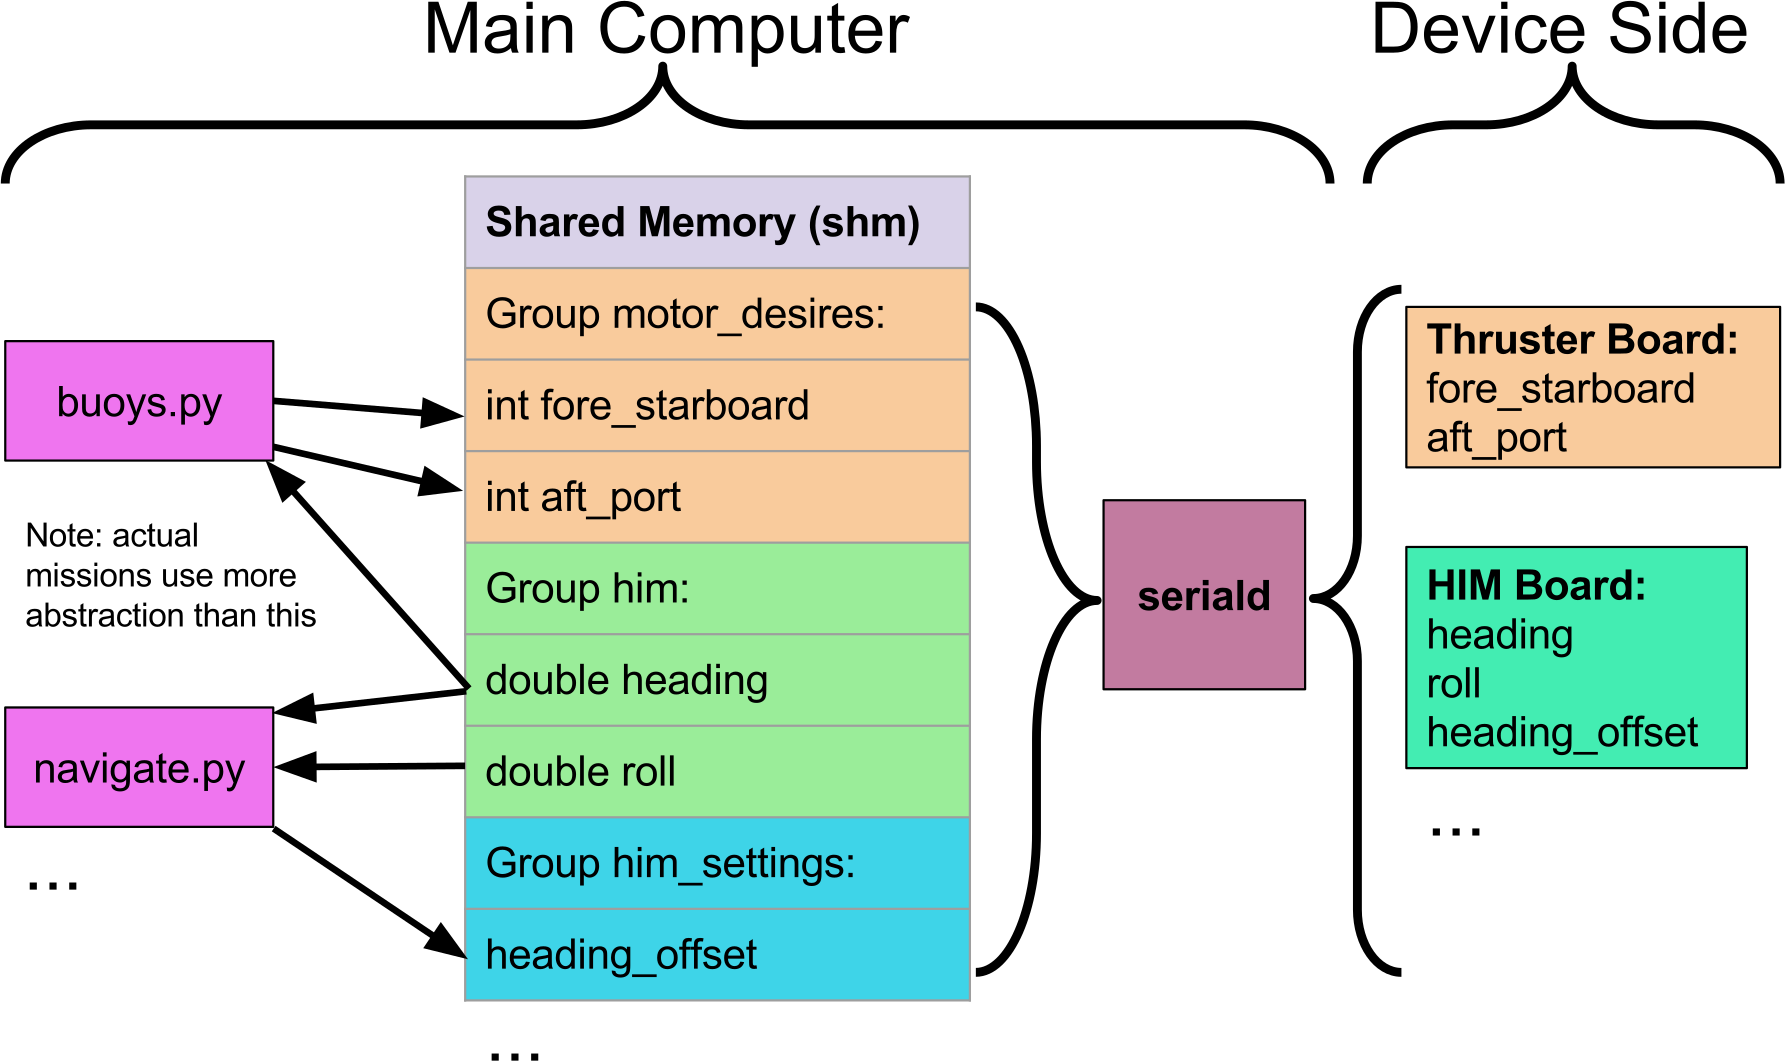
\includegraphics[width=\textwidth]{images/seriald-context.png}
    \caption{Serial Daemon Context}
    \label{fig:why-seriald}
\end{figure}

Figure \ref{fig:why-seriald} shows how a serial daemon (seriald) facilitates communication between the main computer and serial devices. Programs running on the main computer, such the controller and various missions, write values to variables in shm which are then written to devices by seriald. Likewise, when devices modify their internal variables, seriald reads their values and writes them to corresponding values in shm, allowing programs on the main computer to access them. Seriald must enable any number of devices to read from and write to any number of shm variables across any number of shm groups.

\subsection{Old Serial Stack}

\begin{figure}
    \centering
    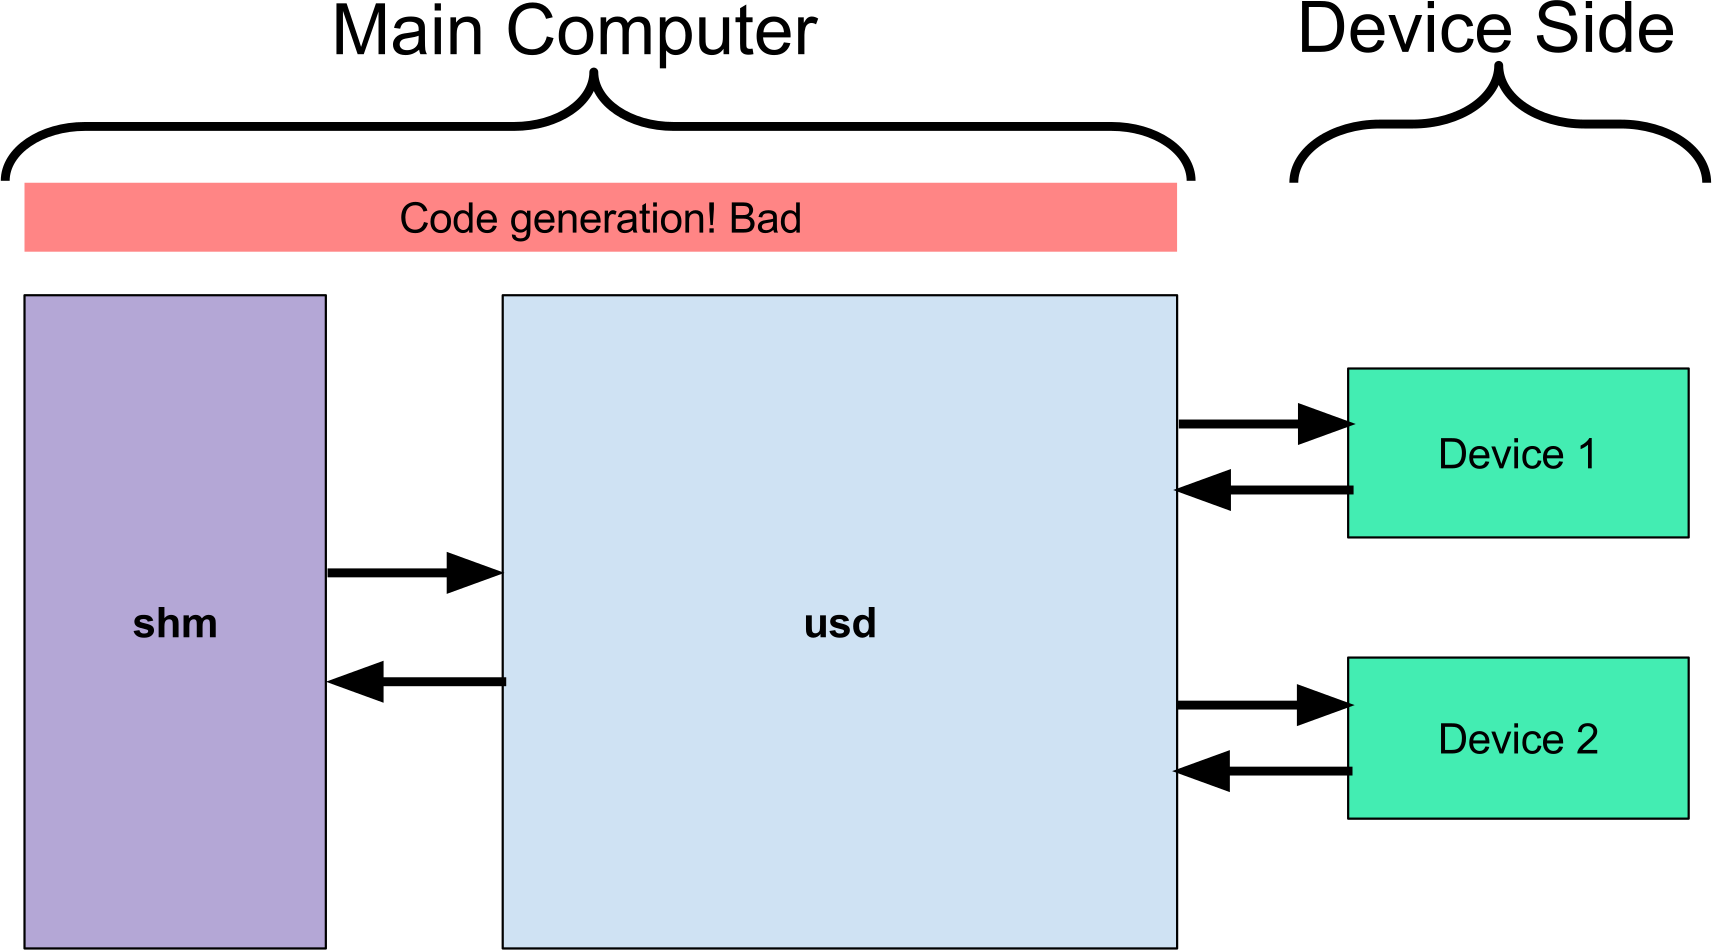
\includegraphics[width=\textwidth]{images/seriald-old-serial.png}
    \caption{Old Serial Overview}
    \label{fig:old-serial}
\end{figure}

Prior to this semester, we used a serial stack known as the universal serial daemon (usd). Although it did function, it had some issues.

\begin{itemize}

\item As depicted in Figure \ref{fig:old-serial}, usd alone handled all communication with shm and serial devices itself. As a consequence, usd was very monolithic; since it implemented both shm communication and serial device communication, other programs which needed to communicate with devices, such as the serial debugger, had to be written from scratch.

\item Since it communicated directly with shm using arbitrary variable and group names, and because the shm API relies on statically generating C structs at compile time, usd also had to be statically generated at compile time. This introducted further code bloat into usd, making it hard to modify, debug, and reason about.

\item Usd was found to have robustness issues. One problem was that it failed to notify shm watchers a single time after updating multiple variables in a group, which was confusing for shm clients.

\item Usd could not reconnect devices after they disconnected, meaning usd had to be restarted in its entirety when devices erroneously disconnected.

\end{itemize}

\section{New Serial Stack}

\subsection{Overview}

\begin{figure}
    \centering
    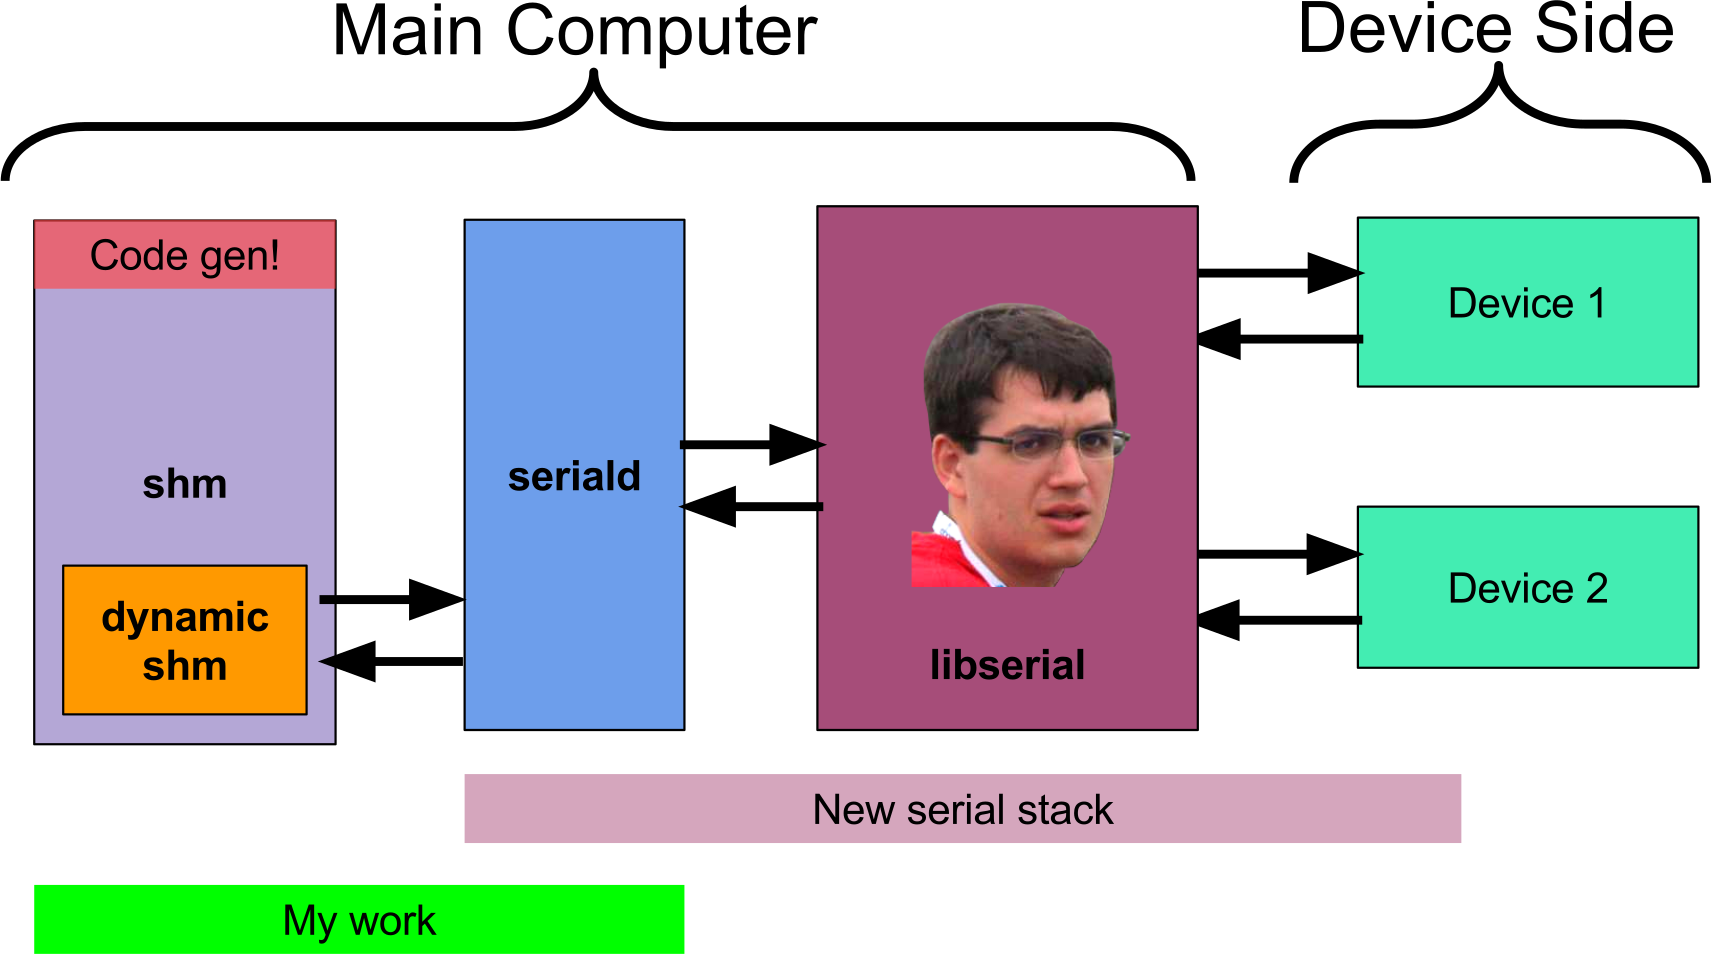
\includegraphics[width=\textwidth]{images/seriald-new-serial.png}
    \caption{New Serial Overview}
    \label{fig:new-serial}
\end{figure}

Figure \ref{fig:new-serial} depicts my work this semester in the context of the new modular serial stack. All direct communication with devices has been refactored into libserial, a library which lets clients send and receive variables to serial devices on a per-port basis. Both libserial and serial devices implement a new serial communication protocol, so the firmware on devices was also updated as a result of introducing a new serial stack. Other utilities, like serial debugger, use libserial to communicate with devices.

My project, new seriald, syncs shm variables with device variables using libserial. To avoid having to statically generate seriald to use shm like usd, I also wrote dynamic shm, an extension to shm which allows C++ programs to use strings to access groups and variables. This allows seriald to be written such that it never needs to directly access shm structs, so it does not need to be statically generated every time shm changes.

\subsection{Dynamic Shm}
\begin{figure}
    \centering
    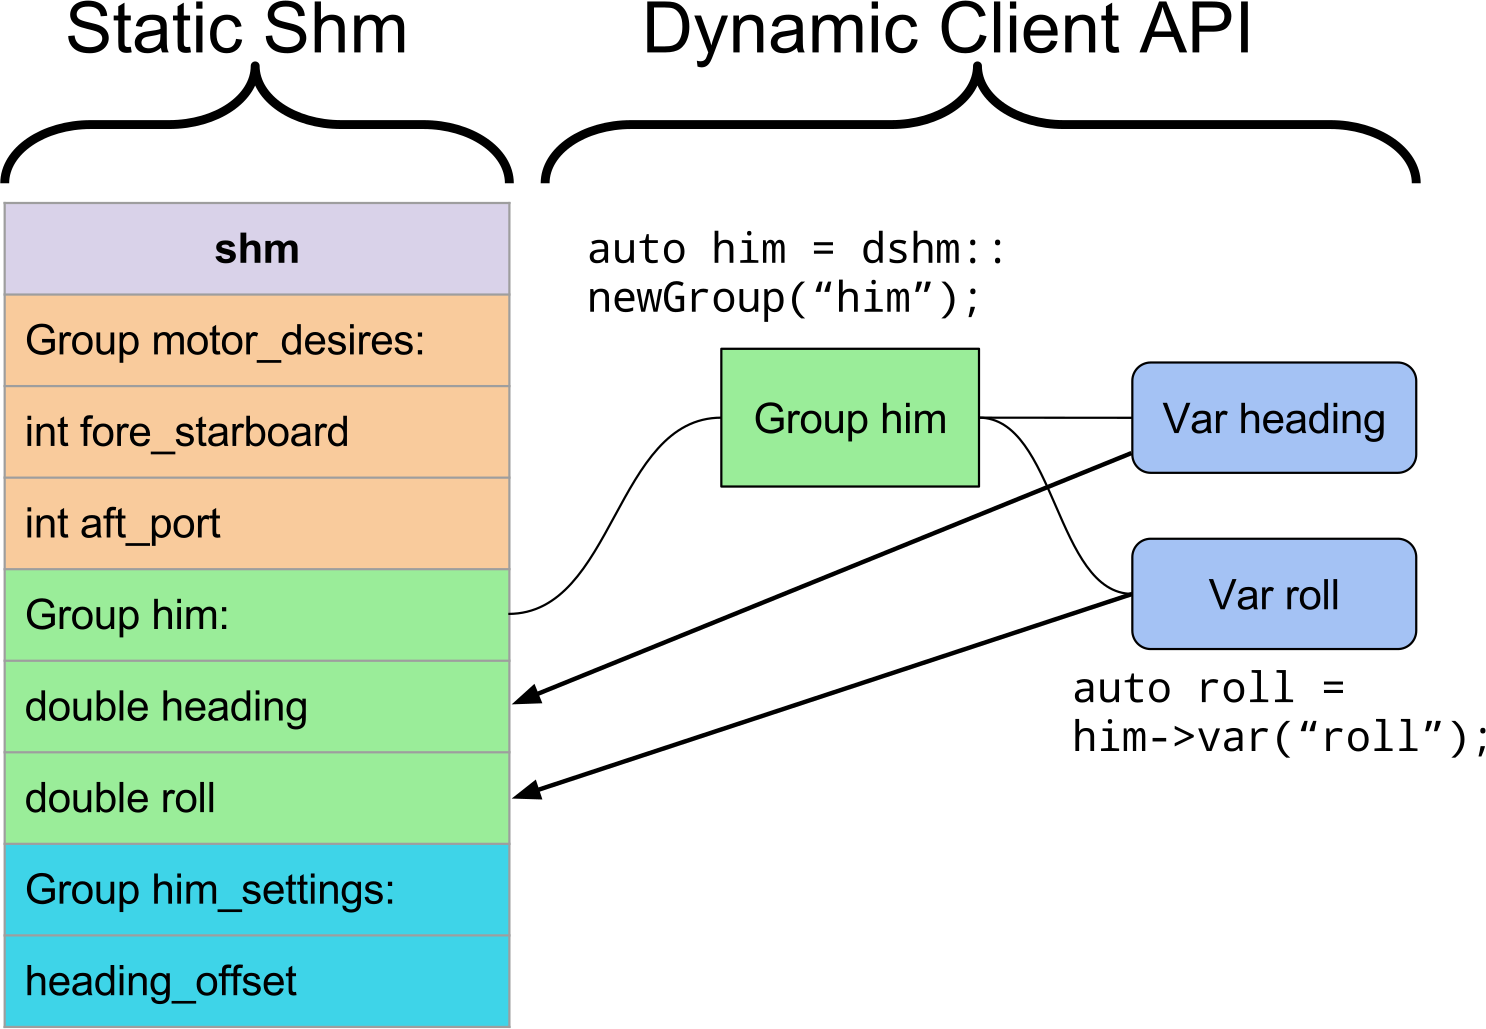
\includegraphics[width=\textwidth]{images/seriald-dynamic-shm.png}
    \caption{Dynamic Shm Overview}
    \label{fig:dynshm}
\end{figure}

Dynamic shm allows clients to read and manipulate shm by specifying the names of variables and groups using strings. To accomplish this, dynamic shm is generated alongside static shm according to the structure specified in vars.conf. Dynamic shm generates one Var subclass for each type of shm variable, including int, double, string, and boolean. Then, it generates one Group subclass for each shm group whose constructor assembles a list of variable class objects which correspond to the shm group's struct fields. Finally, dynamic shm provides a \texttt{newGroup()} method which constructs a Group object linking to the shm group name passed as a parameter.

Group classes expose pointers to their Var objects so clients can efficiently access the same shm variables multiple times. Exposing Var objects is especially useful for seriald since it can construct mappings from libserial variables to shm variables and vice-versa, eliminating the need for large conditional statements when syncing variables. Another useful feature dynamic shm provides is the ability to cache variable writes before writing them to shm. Var classes provide an API for writing to a cache instead of shm, and Group classes provide a \texttt{push()} method which writes only these cached changes to the associated shm group. The \texttt{push()} method leaves unmodified variables untouched, and it only fires shm watchers associated with the group a single time. This atomic behavior prevents potential bugs involving reading only a portion of simultaneously-updated device variables. Similar to the \texttt{push()} method, Group classes additionally provide a \texttt{pull()} method which writes the values of changed group variables to their respective Var caches.

\subsection{Seriald Overview}

\begin{figure}
    \centering
    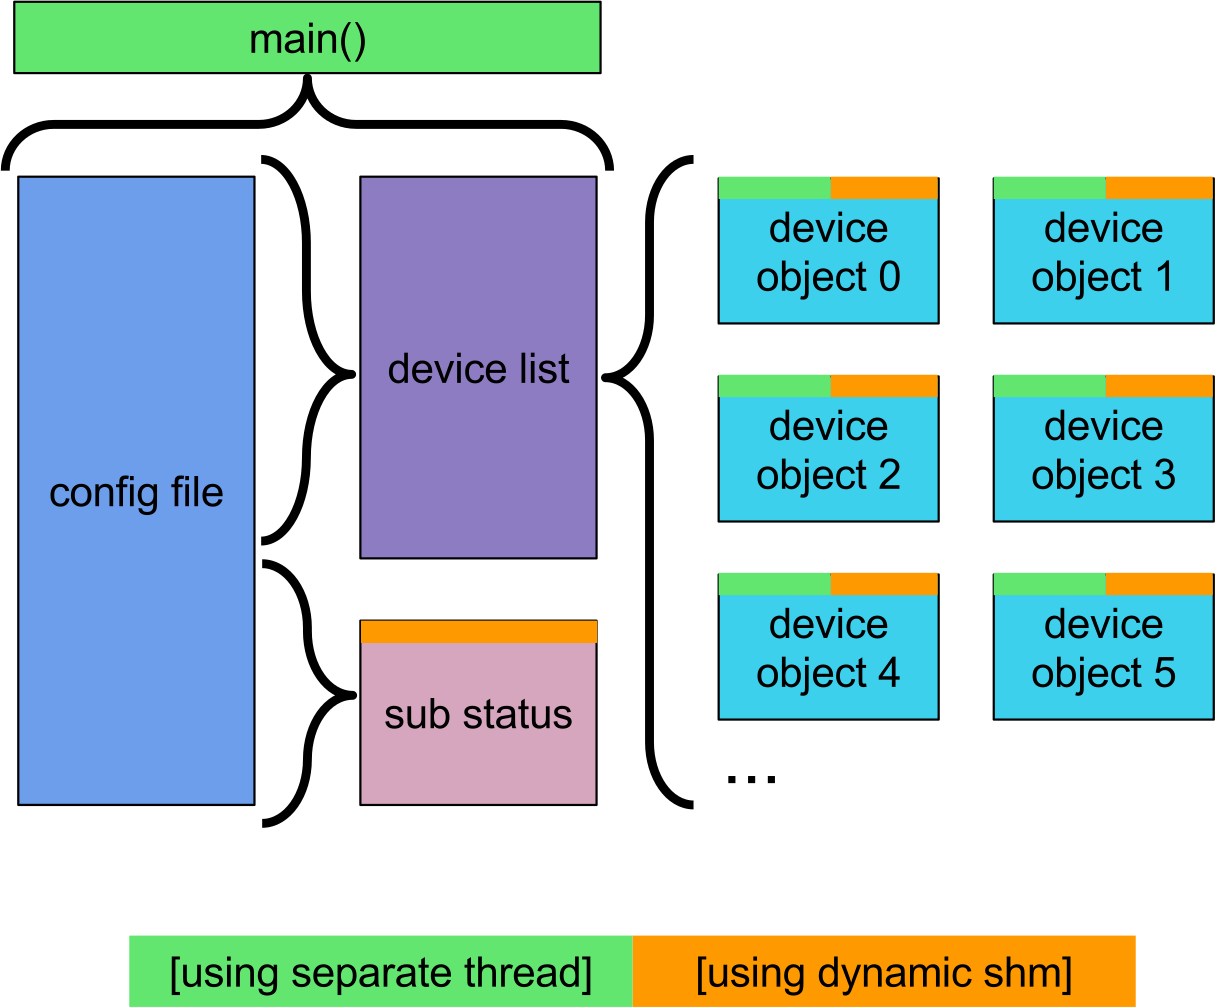
\includegraphics[width=\textwidth]{images/seriald-overview.png}
    \caption{Seriald Implementation Overview}
    \label{fig:overview}
\end{figure}

Seriald uses dynamic shm and libserial to sync variables between shm and serial devices. Figure \ref{fig:overview} depicts the overall structure of seriald.

\begin{itemize}

\item A Config object reads which shm variables should be mapped to which device variables from seriald configuration files. These files are written in TOML (Tom's Obvious Minimal Language), a data serialization format that is easy for humans to read and write.

\item Each serial device is associated with a Device object, each of which contains a thread to read changes from shm and logic to write changes to shm when libserial reports changes in a device's variables. Device objects pass strings parsed from the config files to dynamic shm in order to access the correct variables and groups.

\item A SubStatus object also uses dynamic shm to report which devices are currently connected. It also implements consensus hardkill, which hardkills or unhardkills the sub only when the majority of hardkill-capable devices report such a state. This helps prevent a faulty hardkill mechanism in a device from unintentionally hardkilling the sub.

\item A DeviceList object links device connection callbacks to Device objects, and gracefully handles device disconnections.

\end{itemize}

\begin{figure}
    \centering
    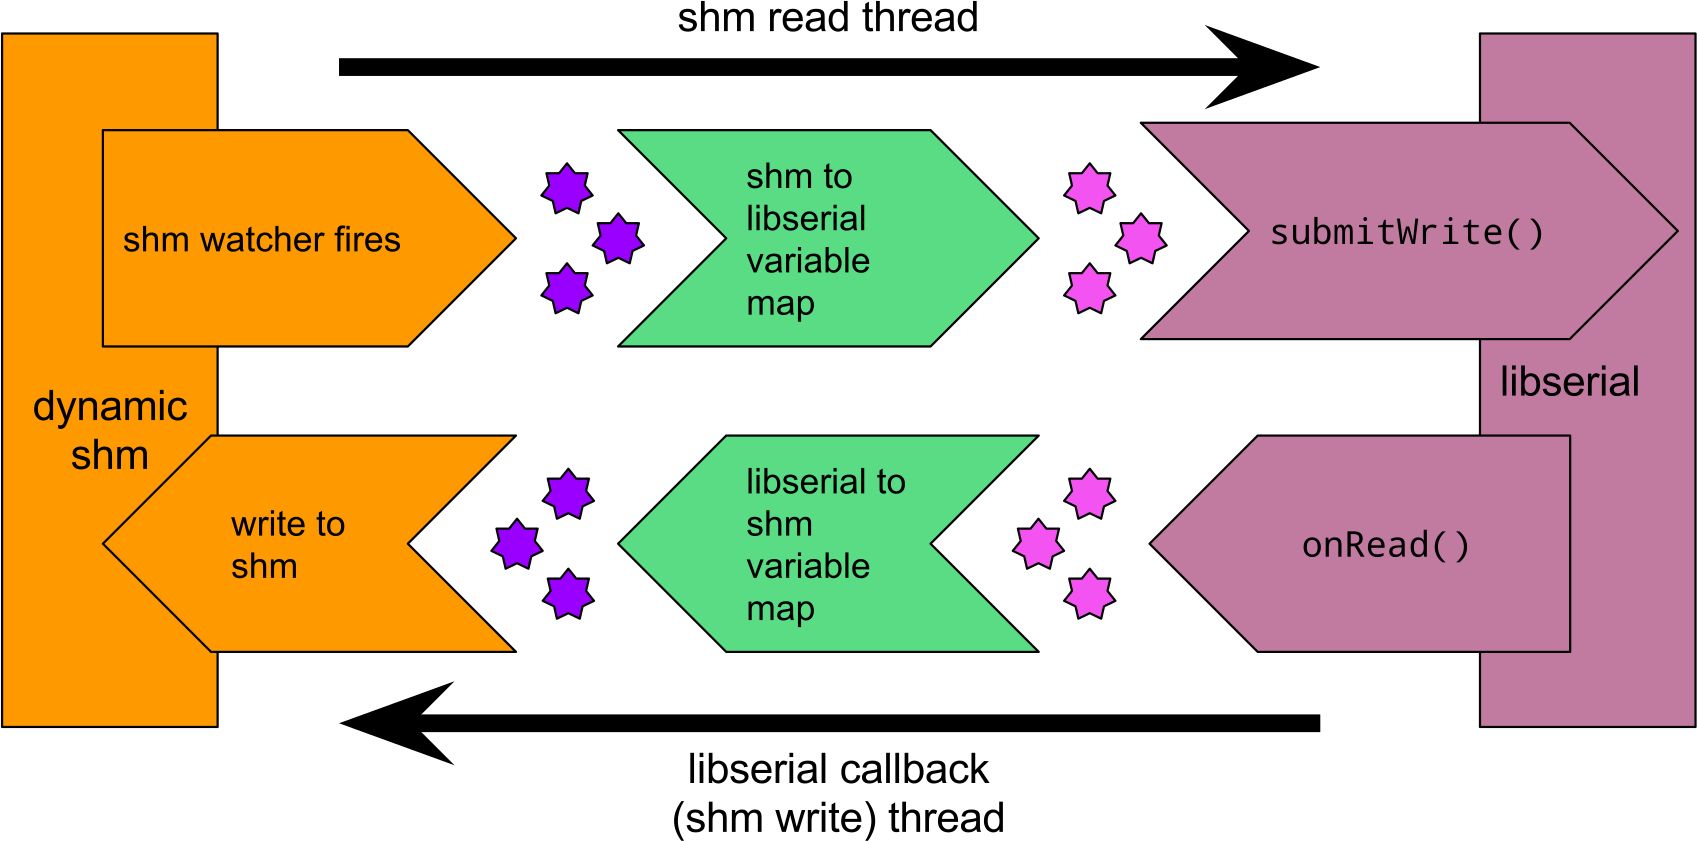
\includegraphics[width=\textwidth]{images/seriald-device-objects.png}
    \caption{Device Objects Implementation Overview}
    \label{fig:device-objects}
\end{figure}

As depicted in Figure \ref{fig:device-objects}, threads running in Device objects use maps to write shm variables to devices and vice-versa. When a shm watcher fires, a shm read thread maps the dynamic shm variables which changed to libserial variables, which are subsequently written to libserial and thus to the correct device. When libserial indicates a device's variables have changed, the containing libserial variables are mapped back to dynamic shm variables, which are written to shm.

\subsection{Seriald Configuration}

On startup, seriald reads shm-device variable mappings, serial port names, and other options from configuration files written in TOML. It begins by reading from the configuration file whose name corresponds with the value of the \texttt{CUAUV\_VEHICLE} environment variable.

\begin{listing}
\begin{minted}{javascript}
includes = [
	"actuator.toml",
	"gpio.toml",
	"him.toml",
	"merge.toml",
	"powerDistribution.toml",
	"thruster.toml",
]

ports = [
	"/dev/ttyUSB_thor_ACT",
	"/dev/ttyUSB_thor_GPIO",
	"/dev/ttyUSB_thor_PD",
	"/dev/ttyUSB_thor_POD",
	"/dev/ttyUSB_thor_THRUST"
]
\end{minted}
\caption{\texttt{thor.toml}, Example Top-Level Config}
\label{listing:top-config}
\end{listing}

Listing \ref{listing:top-config} shows the configuration file seriald would read if \texttt{CUAUV\_VEHICLE} were set to \texttt{thor}. This \texttt{thor.toml} file contains a list of ports to listen to via libserial as well as other configuration files to read, each containing configuration for one device. Modularizing configuration files makes them easier to maintain and allows multiple top-level configuration files to include the same device configuration file. Any configuration file may specify any number of devices, ports, or includes, so long as a circular dependency is not created.

\begin{listing}
\begin{minted}{ini}
[devices.merge.vars]
VehicleCurrent = "merge_status.total_current"
VehicleVoltage = "merge_status.total_voltage"
CurrentA = "merge_status.current_starboard"
CurrentB = "merge_status.current_port"
VoltageA = "merge_status.voltage_starboard"
VoltageB = "merge_status.voltage_port"
MissionStart = "merge_status.mission_start"
MissionLED = "merge.mission_led"

[devices.merge.options]
canHardKill = false
\end{minted}
\caption{\texttt{merge.toml}, Example Device Config}
\label{listing:device-config}
\end{listing}

Listing \ref{listing:device-config} shows \texttt{merge.toml}, a configuration file for merge board. In the \texttt{devices.merge.vars} table, it maps device variable names on the left to paths to shm variables. Device-specific options are set in the \texttt{devices.merge.options} table; in this case, \texttt{canHardKill = false} tells seriald to ignore merge board's hardkill requests.

Including another configuration file essentially merges the child configuration's \texttt{devices} and \texttt{ports} tables with the parent's.

\section{Looking Forward}

The new serial daemon gracefully manages serial connections by itself, yet it does not yet support fine-grained control of its behavior at runtime. It is currently impossible to, for instance, request seriald to temporarily stop communicating with a device so that another program like serial debugger can communicate with it. This could be solved by implementing an IPC scheme in seriald, allowing it to receive commands to direct its behavior.

\end{document}